\documentclass[12pt]{article}

% Packages
\usepackage{amsmath,amssymb}
\usepackage[margin=1in]{geometry}
\usepackage{hyperref}
\usepackage{graphicx}
% Operators
\DeclareMathOperator*{\argmax}{arg,max}

% Document Information
\title{Solving Sudoku with Gradient Descent: An Intuitive Guide}
\author{Jack Vu and Armaan Talabi}
\date{May 2025}

\begin{document}
\maketitle
\section*{Theory}
In multivariable calculus, gradient descent can be used to find the minimum of a function by continuously moving in the direction of the negative gradient. A key point to understand is that the gradient points in the direction of maximum increase; therefore, the negative gradient will point in the direction of the maximum decrease.
\subsection*{Trivial Example}
We can demonstrate gradient descent with a trivial example. For example, we can use gradient descent to minimize some multivariable function. Consider the function $f(x, y) = x^2y$. We can take the partial derivatives of this function to obtain $\frac{\partial f}{\partial x} = 2xy$ and $\frac{\partial f}{\partial y} = x^2$. We know that the gradient of the function is then $\nabla f = (2xy, x^2)$.

Now, imagine that the surface of the graph is a hill. If you are at some initial position $(x, y)$, then you want to take a step in the direction of a negative slope if you want to reach a minimum. Mathematically, this means you should move by some amount in the direction of the negative gradient. Therefore, you should take your initial position and subtract the gradient times some amount, or learning rate $\eta$. You want smaller values of $\eta$ though because you don't want to overshoot the minimum. Using all of this information, we can construct a gradient descent update:

\[(x_{new}, y_{new}) = (x, y) - \eta \nabla f(x, y)\]

\subsection*{Example}
Consider the function $f(x, y) = x^2 + y^2$. The partial derivatives are $\frac{\partial f}{\partial x} = 2x$ and $\frac{\partial f}{\partial y} = 2y$. Therefore, the gradient vector is $(2x, 2y)$. Say you start at the point $(2, 2)$ and you want to use gradient descent to deduce where the location of the minimum is. Applying the previously derived gradient descent formula:
\[(x_{new}, y_{new}) = (2, 2) - \eta \nabla f(2, 2)\]
We can let $\eta = 0.1$ for simplicity. The gradient of $f$ evaluated at the initial position $(2, 2)$ is $(2(2), 2(2)) = (4, 4)$. Multiplying this by $\eta$ gives $(0.4, 0.4)$. Therefore, the next point is $(1.6, 1.6)$. Of course, repeating this process multiple times will get you closer and closer to the minimum value of $(0, 0)$.

\section*{Application}

In multivariable calculus, gradient descent can be used to find the minimum of a function by continuously moving in the direction of the negative gradient. A key point to understand is that the gradient points in the direction of maximum increase; therefore, the negative gradient will point in the direction of the maximum decrease. We can extend this principle to real-world problems, where we transform a problem into a function of multiple variables that we then minimize.
In our case, we are converting creating a continouous ''loss'' function from the information of all 81 tiles in a Sudoku board, and then computing the gradient to navigate towards a solved board.
\section{Trying to Represent Each Cell Continuously}

For every grid position expressed as some position $(r,c)$, we want to represent the digit $x_{r,c}$ as a continuous variable. The best way we found to do this was with a length-9 vector $\mathbf x_{r,c}=(x_{r,c,1},\dots,x_{r,c,9})$ where $x_{r,c,d}$ is the probability that cell $(r,c)$ contains digit $d$. The sum of the entries in this vector must equal 1. This is similar to the output of a neural network, that provides a probability distribution over the possible digits when identifying a digit in an image, for example. 
To create this vector, though, takes a few steps
First, we need to create a vector of \textit{logits}, which are unbounded real numbers. The magnitude of these logits represents the confidence of the model in that digit being the correct one. Naturally, we then run these logits through the softmax function to convert them into a probability distribution (where the sum of the entries equals 1 and each entry represents the probability of that digit being the correct one).

This is what the softmax function looks like:
\begin{equation}
    p_{r,c,d} = \frac{e^{z_{r,c,d}}}{\sum_{k=1}^{9}e^{z_{r,c,k}}}, \qquad d=1,\dots,9.
\end{equation}
A large $z_{r,c,5}$, for example, makes digit~5 likely in that cell.

\textbf{Predicted digit (for measuring error).}
Instead of picking the largest probability immediately, we use an \emph{expected value}
\begin{equation}
    \hat x_{r,c} = \sum_{d=1}^{9}d\,p_{r,c,d}.
\end{equation}
If $p_{r,c}=\bigl(0,0,0,0,0.9,0.1,0,0,0\bigr)$ then $\hat x\approx5.1$. We use the expected value when computing the error because it gives us a smooth, differentiable way to measure how far off a prediction is from the correct value.
For example, if the model is very confident that the cell is a 5, then $\hat{x} \approx 5.1$, which is close to 5, and the squared error is small.


\section{Step 2 -- Designing the loss function}

Our loss $L$ penalises four kinds of mistakes. All terms are simple sums of squares,
which makes their derivatives easy.
\begin{align*}
    L = \;&\underbrace{w_{\text{giv}}\sum_{(r,c)\in G}(\hat x_{r,c}-g_{r,c})^{2}}_{\text{respect the given clues}} \\
    &+ w_{\text{row}}\sum_{r=1}^{9}\sum_{d=1}^{9}\bigl(\textstyle\sum_c p_{r,c,d}-1\bigr)^{2} \\
    &+ w_{\text{col}}\sum_{c=1}^{9}\sum_{d=1}^{9}\bigl(\textstyle\sum_r p_{r,c,d}-1\bigr)^{2} \\
    &+ w_{\text{sub}}\sum_{b=1}^{9}\sum_{d=1}^{9}\bigl(\textstyle\sum_{(r,c)\in b} p_{r,c,d}-1\bigr)^{2}.
\end{align*}

\begin{itemize}
    \item $G$ is the set of coordinates that come pre-filled in the puzzle with values $g_{r,c}$.
    \item The inner sums count how many times digit~$d$ appears in each row, column, or
          3$\times$3 block and compare that count to~1.
\end{itemize}

\medskip
\noindent\textbf{Weight choice.} In practice $(w_{\text{giv}}, w_{\text{row}}, w_{\text{col}}, w_{\text{sub}}) = (20, 1, 1, 1)$ gives the right balance: 
clues dominate early optimisation; row/column/block rules clean things up later.

\section{Step 3 -- Gradient descent loop}
\begin{enumerate}
    \item \textbf{Initialisation.} Set every entry of $\mathbf z$ to zero except for
          fixed clues. For a clue like ``row 1, col 2 = 3'' we set $z_{1,2,3}=+10$ and
          all other logits in that cell to $-10$; this essentially locks the clue in.
    
    \item \textbf{Iterate.}
          \begin{equation*}
              \mathbf z \leftarrow \mathbf z - \eta_k \nabla_{\mathbf z} L, \qquad
              \eta_k = \frac{\eta_0}{1+0.01k}, \quad \eta_0=1.5.
          \end{equation*}

          where $\eta_k$ is the learning rate, which we decrease over time to allow for the model to converge smoothly. Sort of like step size in Euler's method.
        The gradient computation requires careful application of the chain rule for each term in the loss function:

        1. \textbf{Given Clues Term:} For $(r,c) \in G$:
           \begin{align*}
           \frac{\partial L_{\text{giv}}}{\partial z_{r,c,d}} &= w_{\text{giv}} \cdot 2(\hat x_{r,c}-g_{r,c}) \cdot \frac{\partial \hat x_{r,c}}{\partial z_{r,c,d}} \\
           &= w_{\text{giv}} \cdot 2(\hat x_{r,c}-g_{r,c}) \cdot \sum_{k=1}^9 k \cdot \frac{\partial p_{r,c,k}}{\partial z_{r,c,d}} \\
           &= w_{\text{giv}} \cdot 2(\hat x_{r,c}-g_{r,c}) \cdot \sum_{k=1}^9 k \cdot p_{r,c,k}(\delta_{dk} - p_{r,c,d})
           \end{align*}

        2. \textbf{Row Constraint Term:} 
           \begin{align*}
           \frac{\partial L_{\text{row}}}{\partial z_{r,c,d}} &= w_{\text{row}} \cdot 2\left(\sum_{c'} p_{r,c',d}-1\right) \cdot \frac{\partial p_{r,c,d}}{\partial z_{r,c,d}} \\
           &= w_{\text{row}} \cdot 2\left(\sum_{c'} p_{r,c',d}-1\right) \cdot p_{r,c,d}(1-p_{r,c,d})
           \end{align*}

        3. \textbf{Column and Subgrid Terms:} Follow similar patterns, with sums over rows or 3×3 blocks respectively:
           \begin{align*}
           \frac{\partial L_{\text{col}}}{\partial z_{r,c,d}} &= w_{\text{col}} \cdot 2\left(\sum_{r'} p_{r',c,d}-1\right) \cdot p_{r,c,d}(1-p_{r,c,d}) \\
           \frac{\partial L_{\text{sub}}}{\partial z_{r,c,d}} &= w_{\text{sub}} \cdot 2\left(\sum_{(r',c')\in b} p_{r',c',d}-1\right) \cdot p_{r,c,d}(1-p_{r,c,d})
           \end{align*}

    \item \textbf{Stopping.} Quit when $L<10^{-6}$ or after 5000 iterations. If the
          algorithm stagnates, add a bunch of random noise to $\mathbf z$ and
          restart; this usually shakes us out of a shallow local minimum.
    
    \item \textbf{Read out the board.} At convergence, each $p_{r,c}$ is nearly
          one-hot. Pick the index of its largest entry.
\end{enumerate}

\subsection{Credit}
Huge help from Geeks for Geeks explaining softmax and calculating the gradient of the loss function. This was the hardest part. 

\url{https://www.geeksforgeeks.org/derivative-of-the-softmax-function-and-the-categorical-cross-entropy-loss/}

The solver reaches a perfect board after its 5000 iterations ($\approx$2.203 s on a
laptop). The loss curve quickly diminishes, showing that the descent works well!

\begin{figure}[h]
      \centering
      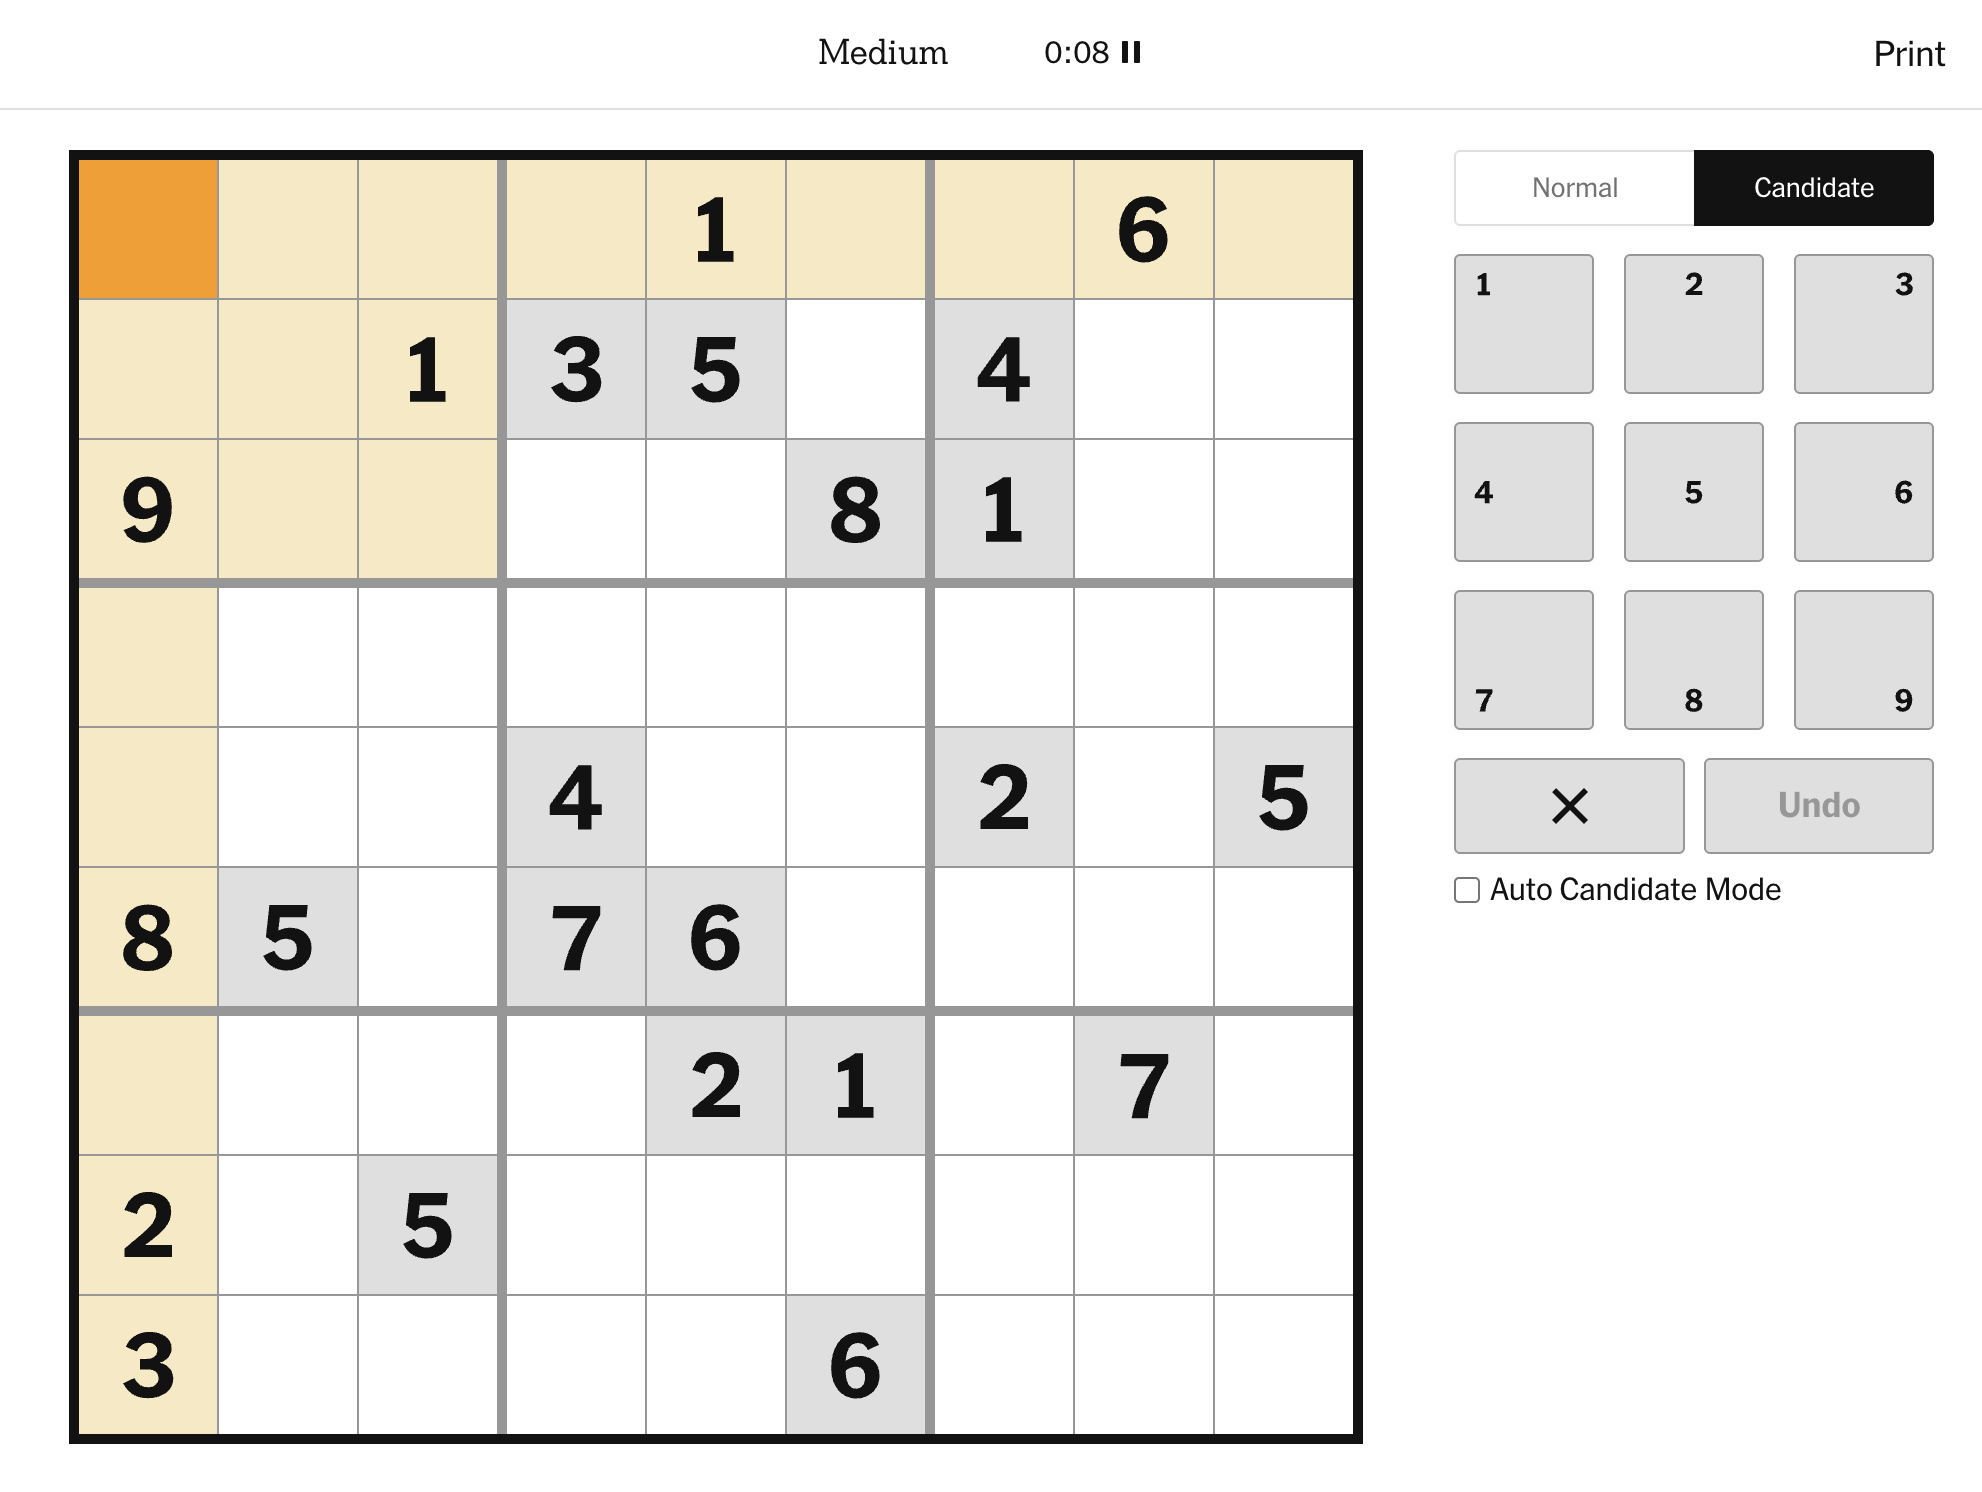
\includegraphics[width=0.4\textwidth]{medium.png}
      \caption{NYT Medium Sudoku Puzzle (Source: New York Times)}
      \label{fig:medium}

      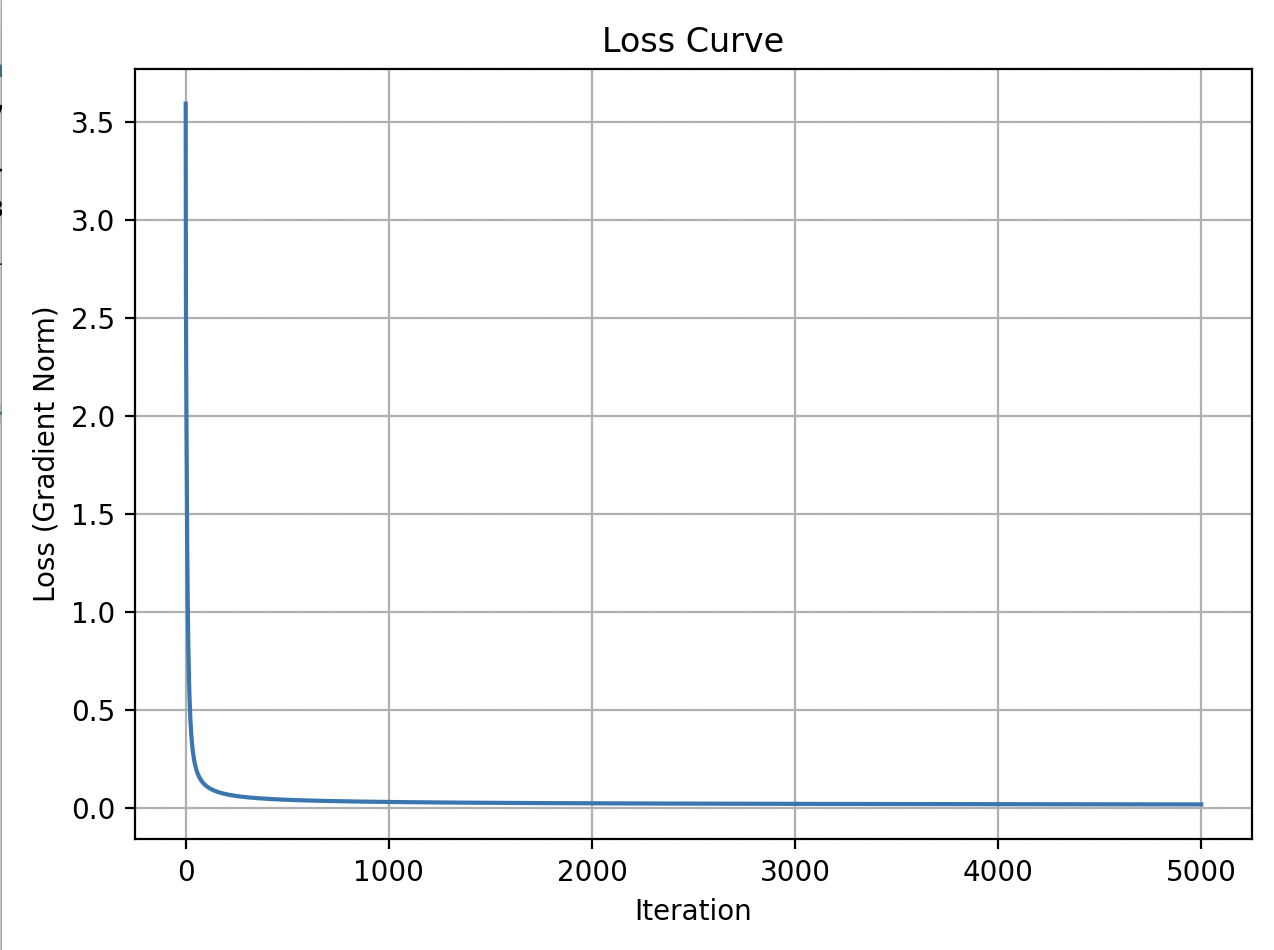
\includegraphics[width=0.4\textwidth]{loss.png}
      \caption{Loss over iterations}
      \label{fig:loss}

      \setlength{\fboxsep}{0pt}
      \setlength{\fboxrule}{1pt}
      \fbox{
\includegraphics[width=0.4\textwidth]{results.png}}
            \caption{Results}
            \label{fig:results}

      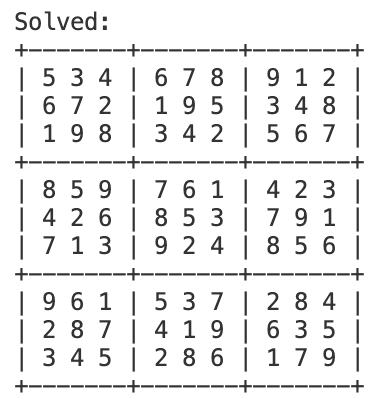
\includegraphics[width=0.4\textwidth]{solved.png}
      \caption{Solved puzzle}
      \label{fig:solved}

\end{figure}

\end{document}
